% vim: set tw=0:
\documentclass{beamer}
\usepackage{graphicx}

% Reasonable themes:
% Antibes Bergen Berkeley Berlin Frankfurt Goettingen Ilmenau Luebeck Malmoe
% Montpellier PaloAlto Rochester Singapore Szeged Warsaw bars boxes
% compatibility default lined plain shadow sidebar split tree
% And these ones include the author's name on every slide:
% Berkeley

% Declare themes.
\mode<presentation>
\usetheme{UWHEP}

% Personal macros.
\newcommand{\email}[1]{{\texttt #1}}
\newcommand{\newframe}[1]{\section{#1}
    \frametitle{\sc{#1}}}
\newcommand{\subframe}[1]{\subsection{#1}
    \frametitle{\sc{#1}}}
\newcommand{\supers}[1]{\ensuremath{^\textrm{#1}}}
\newcommand{\subs}[1]{\ensuremath{_\textrm{#1}}}
\newcommand{\ca}{\ensuremath{\sim}}

% Author information.
\title{T2 Status}
\author[Maier, Mohapatra]{
    Will Maier \and Ajit Mohapatra\\ 
    {\tt wcmaier@hep.wisc.edu}\\
    {\tt ajit@hep.wisc.edu}}
\institute[Wisconsin]{University of Wisconsin - High Energy Physics}
\date{2008.01.22}
\logo{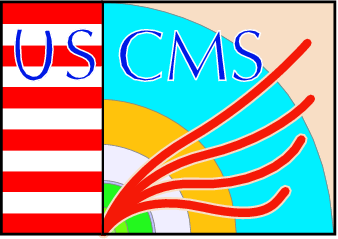
\includegraphics[height=0.6cm]{../../../Graphics/USCMS_logo.png}\hspace{.1cm}
\includegraphics[height=0.75cm]{../../../Graphics/UW_logo.png}}

\begin{document}

\begin{frame}
    \titlepage
\end{frame}

%\section{Overview}
%\begin{frame}
%    \tableofcontents
%\end{frame}

\section{Facilities}
\subsection{Software and Storage}
\begin{frame}
\frametitle{Post-upgrade problems}
\begin{itemize}
    \item Observed severe PNFS performance problems after upgrade
    \begin{itemize}
        \item PNFS manager processed messages at a very low rate
        \item Recompilation of PnfsManager 1.42 (proposed by Brian) resolved issue
        \item Regression introduced in dCache 1.8-9 fixed in 1.8-12?
        \item Will test 1.8-12 this week
    \end{itemize}
    \item {\tt srm-advisory-delete} broken at Wisconsin in 1.8
    \begin{itemize}
        \item Noticed when SAM stageout tests began failing after upgrade (stageout suceeds, but incidental removal fails)
        \item Appears to work at other sites running 1.8
        \item Timur suggested that the brokenness might be due to an out-of-sync .jar, but our installation is clean
        \item At a bit of a dead end
    \end{itemize}
    \item Despite problems, Wisconsin dCache is (at least) usable since the PNFS fix
    \item New server hardware on order
\end{itemize}
\end{frame}

\subsection{Production and Monitoring}
\begin{frame}
\frametitle{}
\begin{itemize}
    \item JobRobot/SAM:
    \begin{itemize}
        \item stageout test fails due to {\tt srm-advisory-delete} brokenness since 1.8 upgrade
        \item Will upgrade dCache to latest patchlevel soon (in case our problem is somehow related to Brian's .jar hack)
    \end{itemize}
    \item LoadTest/PhEDEx:
    \begin{itemize}
        \item Transfers from IN2P3 are unstable
        \item RAL transfers finally exceeded 300GB/day today (is Nebraska still downloading?)
    \end{itemize}
    \item Production
    \begin{itemize}
        \item Mike Anderson will run production for the next month
        \item Running one of 2x10M CSA07 requests with CMSSW\_174
        \item Production slowed by large CMSSW\_174 memory footprint and reliance on Squid databases for calibration data
        \item Memory problems should be fixed in CMSSW\_18X, but will persist with CMSSW\_17X
        \item What to do? Should we reduce the number of batch slots on each worker node? Other options?
    \end{itemize}
\end{itemize}
\end{frame}

\end{document}
